\documentclass[11pt]{article}
\usepackage{mathtools}
\usepackage{amsmath}
\usepackage{amssymb}
\usepackage{amsfonts}
\usepackage{amsthm}
\usepackage{xcolor}
\usepackage{graphicx}
\usepackage[top=2.0cm,bottom=2.0cm,left=2.5cm,right=2.5cm]{geometry}
\usepackage{tikz}
\usepackage{float}
\usepackage{multicol}
\usepackage{pgfplots}
\usepackage{lastpage}
\usepackage{siunitx}
\usepackage{xspace}
\usepackage[labelfont=bf]{caption}
\usepackage[hidelinks, urlcolor=blue, linkcolor=blue, colorlinks=true]{hyperref}
\usepackage[capitalize,noabbrev]{cleveref}
\usepackage[absolute]{textpos}
\usepackage{systeme}

\newcommand{\R}{\mathbb{R}}
\newcommand{\C}{\mathbb{C}}
%% define course title
\newcommand{\course}{MAT185}
\newcommand{\assignmenttitle}{Assignment 1}

%% header and footer
\firstpageheader{}{}{\textbf{{\color{red} Due:} 10:00pm, Tuesday Jan. 21, 2025}}
\firstpageheadrule
\runningheader{}{Page~\thepage~of~\numpages}{\course~--~\assignmenttitle}
\footer{}{}{}

\setlength\parindent{0pt} % no indentation in document

%% formats exam class
\qformat{\textbf{Question \thequestiontitle:}\hfill} % title of question 
\boxedpoints
\pointpoints{mark}{marks}
\pointsinrightmargin
\hpword{Marks:}
\hsword{Your score:}
\unframedsolutions
\totalformat{\boxed{\textnormal{\totalpoints~\if\totalpoints1 mark\else marks\fi}}}
\definecolor{SolutionColor}{rgb}{0,0,1}
\renewcommand{\solutiontitle}{}
\AtBeginEnvironment{solution}{\color{blue}}

% %correct choices in solution
\CorrectChoiceEmphasis{\rm}
\checkedchar{\tikz\draw[blue,fill=blue] (0,0) circle (1ex);}

% % increase distance between checkbox items
\renewcommand{\checkboxeshook}{\setlength{\itemsep}{6pt}}

%% distance between questions and parts
\renewcommand{\questionshook}{\setlength{\parsep}{10pt}}
\renewcommand{\partshook}{\setlength{\parsep}{15pt}}

%% define arrows in text
\newcommand{\arrow}{$\rightarrow$\xspace}
\newcommand{\Arrow}{$\Rightarrow$\xspace}

% % math notation:
%\veccol{1}{2}{3}
\newcommand{\veccol}[3]{
    \begin{bmatrix}
        #1\\
        #2\\
        #3\\
    \end{bmatrix}}
  
%\vecrow{1}{2}{3}
\newcommand{\vecrow}[3]{\left[#1~#2~ #3\right]}

%\matrixTwo{1}{2}{3}{4}
\newcommand{\matrixTwo}[4]{\left[\begin{array}{cc}#1&#2\\#3&#4\end{array}\right]}

% \matrixThree{1}{2}{3}{4}{5}{6}{7}{8}{9}
\newcommand{\matrixThree}[9]{\left[\begin{array}{ccc}#1&#2&#3\\#4&#5&#6\\#7&#8&#9\end{array}\right]}

%\matrixCorner{1}{2}{3}{4}
\newcommand{\matrixCorner}[4]{\left[\begin{array}{ccc}#1& \cdots&#2\\ \vdots & \ddots & \vdots\\#3&
      \cdots&#4\end{array}\right]}

% \nR
\newcommand{\nR}{{}^{n}\mathbb{R}}
% \Rn
\newcommand{\Rn}{\mathbb{R}^{n}}
% \nRn
\newcommand{\nRn}{{}^{n}\mathbb{R}^{n}}
% \nRm
\newcommand{\nRm}{{}^{n}\mathbb{R}^{m}}
% \nRm
\newcommand{\mRn}{{}^{m}\mathbb{R}^{n}}
% \mRm
\newcommand{\mRm}{{}^{m}\mathbb{R}^{m}}        

% \u
\renewcommand{\u}{{\bf u}}      
% \v
\renewcommand{\v}{{\bf v}}      
% \w
\newcommand{\w}{{\bf w}}    
% \V
\newcommand{\V}{{\bf V}}                   
       
%% define abbreviations
\newcommand{\row}{\operatorname{row}\,}
\newcommand{\col}{\operatorname{col}\,}
\renewcommand{\dim}{\operatorname{dim}\,}
\renewcommand{\span}{\operatorname{span}\,}
\newcommand{\rank}{\operatorname{rank}\,}
\renewcommand{\ker}{\operatorname{ker}\,}
\newcommand{\nul}{\operatorname{null}\,}
\renewcommand{\det}{\operatorname{det}\,}
\newcommand{\adj}{\operatorname{adj}\,}

\usepackage{xcolor}
% Sean's original colours:
%\definecolor{dkrgreen}{rgb}{0.1, 0.4, 0.3} 
\definecolor{dkrgreen}{HTML}{009988} % this is the color-blind friendly teal from below
%\definecolor{dkred}{rgb}{0.8, 0.05, 0.05} 
\definecolor{dkred}{HTML}{EE3377}  % this is the colour-blind friendly magenta from below
%\definecolor{orange}{rgb}{0.8, 0.33, 0.0}
%\definecolor{goldenrod}{rgb}{0.85, 0.65, 0.13}
\definecolor{blue}{HTML}{1965B0} % this is the colour-blind friendly blue from below
%
% colour-blind-friendly colours from https://personal.sron.nl/~pault/
\definecolor{tolBlue}{HTML}{1965B0}
\definecolor{tolMedBlue}{HTML}{5289C7}
\definecolor{tolLightBlue}{HTML}{7BAFDE} 
\definecolor{tolRed}{HTML}{E8601C} 
\definecolor{tolYellow}{HTML}{F6C141}
\definecolor{tolTeal}{HTML}{009988}
%\definecolor{tolBlue}{HTML}{0077BB} 
\definecolor{tolCyan}{HTML}{33BBEE}
\definecolor{tolTeal}{HTML}{009988} 
\definecolor{tolOrange}{HTML}{EE7733} 
%\definecolor{tolRed}{HTML}{CC3311} 
\definecolor{tolMagenta}{HTML}{EE3377} 
\definecolor{tolGrey}{HTML}{BBBBBB}

%%% This command makes a framed box of a chosen height.
\newcommand{\makenonemptybox}[2]{%
\par\nobreak\vspace{\ht\strutbox}\noindent
\setlength{\fboxrule}{0pt} % set this to 0pt to make invisible
\fbox{%
\parbox[c][#1][t]{\dimexpr\linewidth-2\fboxsep}{
  \hrule width \hsize height 0pt
  \vspace{-0.6cm}
  \color{SolutionColor}#2\color{black}
 }%
}%
}


\begin{document}
\thispagestyle{empty}
{\LARGE \bf ESC 195 Lecture Notes}\\
{\large Hei Shing Cheung}\\
Caculus II, Winter 2024 \hfill ESC 195\\
\\
The up-to-date version of this document can be found at \url{https://github.com/HaysonC/skulenotes}\\

\section{More on Integrals}
\subsection{Riemann Sum - Non-Uniform Petition}
\begin{example}
    Given the following definite integral:
    $$\int^2_0 \sqrt{x} dx$$, we cannot evaluate its Riemann sum with uniforms partition, since the series of root cannot be easily evaluated. 
\end{example}

The definite integral of $\sqrt{x}$ from $0$ to $2$ using a Riemann sum with a non-uniform partition is given by:

$$\int_{0}^{2} \sqrt{x} \, dx = \lim_{n \to \infty} \sum_{i=1}^n \sqrt{x_i} \Delta x_i$$
, where:
\begin{itemize}
    \item $x_0 = 0, \, x_n = 2$,
    \item $x_i = i^2 \cdot \frac{2}{n^2}$ for $i = 0, 1, 2, \dots, n$,
    \item $\Delta x_i = x_i - x_{i-1} = \frac{2}{n^2} \cdot (2i - 1)$.
\end{itemize}

The Riemann sum becomes:
$$
S_n = \sum_{i=1}^n \sqrt{i^2 \cdot \frac{2}{n^2}} \cdot \frac{2}{n^2} \cdot (2i - 1).
$$

Simplifying further:
$$
S_n = \sum_{i=1}^n \sqrt{\frac{2i^2}{n^2}} \cdot \frac{2}{n^2} \cdot (2i - 1).
$$

Taking the limit as $n \to \infty$, the sum converges to the exact value of the integral using the series of squares. 
$$
\int_{0}^{2} \sqrt{x} \, dx = \frac{4\sqrt{2}}{3}.
$$
\paragraph{Condition} $n \to \infty$ Ensures $\Delta x_i \to 0$
\paragraph{} As $n \to \infty$, the partition points $x_i$ become increasingly dense. This ensures that the partition becomes infinitely fine.

\subsection{Integration By Parts}
Using the product rule:
$$
\frac{d}{dx} \big[ u(x) v(x) \big] = u'(x)v(x) + u(x)v'(x),
$$
integrating both sides with respect to $x$ gives:
$$
u(x)v(x) = \int u'(x) v(x) \, dx + \int u(x) v'(x) \, dx.
$$
Rearranging this:
$$\int u'(x) v(x) \, dx = u(x)v(x) - \int u(x) v'(x) \, dx.$$

\paragraph{Integration by parts formula}
\begin{equation}
\int u \, dv = uv - \int v \, du.
\end{equation}
\begin{example}
We want to solve the integral $$ \int x e^{2x} \, dx $$ using integration by parts.

Let:
$$ u = x, \quad dv = e^{2x} \, dx. $$

Then, we compute the derivatives and integrals:
$$ du = dx, \quad v = \frac{e^{2x}}{2}. $$

Now, apply the integration by parts formula:
$$ \int u \, dv = uv - \int v \, du. $$

Substituting in the values:
$$ \int x e^{2x} \, dx = x \cdot \frac{e^{2x}}{2} - \int \frac{e^{2x}}{2} \, dx. $$

Next, compute the remaining integral:
$$ \int \frac{e^{2x}}{2} \, dx = \frac{e^{2x}}{4}. $$

Thus, the result is:
$$ \int x e^{2x} \, dx = \frac{x e^{2x}}{2} - \frac{e^{2x}}{4} + C. $$

\end{example}

\begin{example}
We want to solve $$ \int x^2 \sin(2x) \, dx $$ using double integration by parts.

First, let:
$$ u = x^2, \quad dv = \sin(2x) \, dx. $$

Then:
$$ du = 2x \, dx, \quad v = -\frac{1}{2} \cos(2x). $$

Using the IBP formula:
$$ \int u \, dv = uv - \int v \, du, $$

we get:
$$ \int x^2 \sin(2x) \, dx = -\frac{x^2}{2} \cos(2x) + \int x \cos(2x) \, dx. $$

Now, apply IBP again to \( \int x \cos(2x) \, dx \), let:
$$ u = x, \quad dv = \cos(2x) \, dx. $$

Then:
$$ du = dx, \quad v = \frac{1}{2} \sin(2x). $$

Using the IBP formula again:
$$ \int x \cos(2x) \, dx = \frac{x}{2} \sin(2x) - \int \frac{1}{2} \sin(2x) \, dx, $$

and solving the remaining integral:
$$ \int \frac{1}{2} \sin(2x) \, dx = -\frac{1}{4} \cos(2x). $$

Thus, the final result is:
$$ \int x^2 \sin(2x) \, dx = -\frac{x^2}{2} \cos(2x) + \frac{x}{2} \sin(2x) + \frac{1}{4} \cos(2x) + C. $$

\end{example}
\subsection{Trigonometric Integrals}
\paragraph{Case I} This is the case I trigonometric integrals, the strategy is using the pythagorean identity.
\paragraph{} We want to solve the class of integrals:
\begin{equation}
 \int \sin^n(x) \cos^m(x) \, dx
\end{equation}
, where $m$ or $n$ is odd.
\begin{example}
We want to solve the integral:
$$ I = \int \sin^3(x) \cos^2(x) dx $$
We use the identity: $ \sin^2(x) = 1 - \cos^2(x)$. Thus, the integral becomes:
\begin{align*}
    I &= \int \sin(x)(1 - \cos^2(x)) \cos^2(x) \, dx \\
    &= \int (\cos^2(x) \sin(x) - \cos^4(x) \sin(x)) \, dx
\end{align*} 
which is now easily solvable with substution $u=\cos(x)$.
\end{example}
\paragraph{Case II} The follwoing is generally solvable via case I and case III below. In general, we solve the integral by reducing the power of the trigonometric functions to arrive at a solvable integral Case I or III.
\paragraph{} We want to solve the class of integrals:
\begin{equation} \int \sin^n(x) \cos^m(x) \, dx \end{equation}
, where $m$ and $n$ is even.
\begin{example}
We want to solve the integral:
$$ I = \int \sin^2(x) \cos^4(x) \, dx $$
We can apply the double angle formulas:
\begin{align}
    \sin(x)\cos(x) &= \frac{1}{2} \sin(2x) \\
    \sin^2(x) &= \frac{1 - \cos(2x)}{2} \\
    \cos^2(x) &= \frac{1 + \cos(2x)}{2}
\end{align}
Thus, the integral becomes:
$$ I = \frac{1}{8} \int \sin^2(2x) \, dx + \frac{1}{8} \int \cos(2x)\sin^2(2x) \, dx $$
\end{example}
\paragraph{Case III} This is the case III trigonometric integrals, the strategy is using the reduction formula via IBP.
\paragraph{Reduction Formula} We can solve integrals by reducing the power of the trigonometric functions. These are done using IBP and trigonometric identities.
\paragraph{} We want to solve the classes of integrals:
\begin{equation} 
    \int \sin^n(x) \, dx, \quad \int \cos^n(x) \, dx 
\end{equation}
, where $n$ is a positive integer. For demonstartion, We can obtain the reduction formula of $\sin^n(x)$ via IBP.
\begin{align}
    I_n &= \int \sin^n(x) \, dx \nonumber \\
    &= \int \sin^{n-1}(x) \sin(x) \, dx \nonumber \\
    &= \frac{-\cos(x) \sin^{n-1}(x)}{n} + \frac{(n-1)}{n} \int \cos^2(x) \sin^{n-2}(x) \, dx \nonumber \\
    &= \frac{-\cos(x) \sin^{n-1}(x)}{n} + \frac{(n-1)}{n} I_{n-2}
\end{align}
\paragraph{Reduction for $\cos^n(x)$} We can obtain the reduction formula of $\cos^n(x)$ via IBP.
\begin{align}
    I_n &= \int \cos^n(x) \, dx \nonumber \\
    &= \int \cos^{n-1}(x) \cos(x) \, dx \nonumber \\
    &= \frac{\sin(x) \cos^{n-1}(x)}{n} + \frac{(n-1)}{n} \int \sin^2(x) \cos^{n-2}(x) \, dx \nonumber \\
    &= \frac{\sin(x) \cos^{n-1}(x)}{n} + \frac{(n-1)}{n} I_{n-2}
\end{align} 
\paragraph{Case IV} The following is generally solvable via simple trigonometric integrals. In general, we solve the integral by applying the angle sum formulas.
\paragraph{} We want to solve the classes of integrals:
\begin{equation}
    \int \sin(mx) \cos(nx) \, dx, \quad \int \sin(mx) \sin(nx) \, dx, \quad \int \cos(mx) \cos(nx) \, dx 
\end{equation}
We could apply the angle sum formulas:
\begin{align}
    \sin(mx)\cos(nx) &= \frac{1}{2} \left[ \sin((m+n)x) + \sin((m-n)x) \right] \\
    \sin(mx)\sin(nx) &= \frac{1}{2} \left[ \cos((m-n)x) - \cos((m+n)x) \right] \\
    \cos(mx)\cos(nx) &= \frac{1}{2} \left[ \cos((m-n)x) + \cos((m+n)x) \right]
\end{align}
\paragraph{Case V} The following is generally solvable via the following trigonometric identities listed below, which convert it into a reduction formula.
\begin{align}
    \tan^2(x) &= \sec^2(x) - 1 \label{eq:tan2} \\
    \cot^2(x) &= \csc^2(x) - 1 \label{eq:cot2}  \\
    \frac{d}{dx} \tan(x) &= \sec^2(x)
\end{align}
\paragraph{} We want to solve the classes of integral:
\begin{equation}
    \int \tan^n(x) \, dx, \quad \int \cot^n(x) \, dx 
\end{equation}
We know that $tan^2(x) = \sec^2(x) - 1$. Thus, we can solve the integral by reducing the power of the tangent function.
\paragraph{Reduction for $\tan^n(x)$} We can obtain the reduction formula of $\tan^n(x)$ via the trigonometric identities.
\begin{align}
    I_n &= \int \tan^n(x) \, dx \nonumber \\
    &= \int \tan^{n-1}(x) \tan(x) \, dx \nonumber \\
    &= \frac{\tan^{n-1}(x)}{n-1} - \int \tan^{n-2}(x) \, dx \nonumber \\
    &= \frac{\tan^{n-1}(x)}{n-1} - I_{n-2}
\end{align}
\paragraph{Reduction for $\cot^n(x)$} We can obtain the reduction formula of $\cot^n(x)$ via the trigonometric identities.
\begin{align}
    I_n &= \int \cot^n(x) \, dx \nonumber \\
    &= \int \cot^{n-1}(x) \cot(x) \, dx \nonumber \\
    &= \frac{\cot^{n-1}(x)}{n-1} - \int \cot^{n-2}(x) \, dx \nonumber \\
    &= \frac{\cot^{n-1}(x)}{n-1} - I_{n-2}
\end{align}
\paragraph{Case VI} The following is generally solvable via the trigonometric identities (\ref{eq:tan2}) and (\ref{eq:cot2}).
\paragraph{} We want to solve the classes of integral:
\begin{equation} 
    \int \tan^m(x) \sec^n(x) \, dx, \quad \int \cot^m(x) \csc^n(x) \, dx 
\end{equation}
We can solve the integral by reducing the power of the converted trigonometric functions using (\ref{eq:tan2}) and (\ref{eq:cot2}).
\paragraph{Case VII} The following is generally solvable via the trigonometric identities (\ref{eq:tan2}) and (\ref{eq:cot2}).
\paragraph{} We want to solve the classes of integral:
\begin{equation} \int \tan^m(x) \sec^n(x) \, dx, \quad \int \cot^m(x) \csc^n(x) \, dx \end{equation}
We can solve the integral by converting between the tangent and secant functions using the trigonometric identities.
\paragraph{Case VIII} This is the case VIII integrals, the strategy is using the trigonometric substitution.
\paragraph{Trigonometric Substitution} We can solve integrals by substituting the trigonometric functions with other trigonometric functions.
\begin{example}
We want to solve the integral:
$$ \int \frac{dx}{\sqrt{1 - x^2}} $$
\end{example}
We can substitute $x = \sin(\theta)$, then $dx = \cos(\theta) \, d\theta$. The integral becomes:
$$ \int \frac{\cos(\theta) \, d\theta}{\sqrt{1 - \sin^2(\theta)}} = \int \frac{\cos(\theta) \, d\theta}{\cos(\theta)} = \int d\theta = \theta + C. $$
\paragraph{} In general, we can use the following substitutions:
\begin{itemize}
    \item $x = a\sin(\theta)$ for $\sqrt{a^2 - x^2}$,
    \item $x = a\tan(\theta)$ for $\sqrt{a^2 + x^2}$,
    \item $x = a\sec(\theta)$ for $\sqrt{x^2 - a^2}$.
\end{itemize}
\paragraph{Weierstrass Substitution} We can solve integrals by using the Weierstrass substitution:
\begin{equation}
    \tan\left(\frac{x}{2}\right) = t \Leftrightarrow \cos(x) = \frac{1-t^2}{1+t^2} \quad \sin(x) = \frac{2t}{1+t^2} \quad dx = \frac{2dt}{1+t^2}
\end{equation}
This substitution is useful for solving integrals with trigonometric functions, by converting them into rational functions.
\paragraph{Summary} We can solve trigonometric integrals by using the following strategies:
\begin{table}[h!]
    \centering
    \begin{tabular}{|c|l|}
    \hline
    \textbf{Case} & \textbf{Strategy and General Form} \\ \hline
    I   & Use \(\sin^2(x) + \cos^2(x) = 1\); simplify using substitution. \\
        & General Form: \(\int \sin^n(x) \cos^m(x) dx\), where \(m\) or \(n\) is odd. \\ \hline
    II  & Convert to Case I and Case III using double angle formulas. \\
        & General Form: \(\int \sin^n(x) \cos^m(x) dx\), where both \(m\) and \(n\) are even. \\ \hline
    III & Apply reduction formulas derived via integration by parts. \\
        & General Form: \(\int \sin^n(x) dx\) or \(\int \cos^n(x) dx\). \\ \hline
    IV  & Use angle sum formulas to simplify. \\
        & General Form: \(\int \sin(mx) \cos(nx) dx\). \\ \hline
    V   & Reduce tangent/cotangent powers using \(\tan^2(x) = \sec^2(x) - 1\) and substitution. \\
        & General Form: \(\int \tan^n(x) dx\) or \(\int \cot^n(x) dx\). \\ \hline
    VI  & Convert to Case V via Pythagorean identities. \\
        & General Form: \(\int \tan^m(x) \sec^n(x) dx\) or \(\int \cot^m(x) \csc^n(x) dx\). \\ \hline
    VII & Convert between tangent and secant functions for simplification. \\
        & General Form: \(\int \tan^m(x) \sec^n(x) dx\). \\ \hline
    VIII & Use trigonometric substitution: \(x = a \sin(\theta), a \tan(\theta), a \sec(\theta)\). \\
         & General Form: \(\int \frac{dx}{\sqrt{a^2 - x^2}}, \int \frac{dx}{\sqrt{a^2 + x^2}}, \int \frac{dx}{\sqrt{x^2 - a^2}}\). \\ \hline
    \end{tabular}
    \caption{Strategies and General Forms for Case I-VIII Integrals}
\end{table}
\subsection{Partial Fractions}
\paragraph{Partial Fraction Decomposition} We can decompose a rational function into partial fractions to simplify integration.
\paragraph{} We want to solve the integral:
\begin{equation}
    \int \frac{P(x)}{Q(x)} \, dx
\end{equation}
, where $P(x)$ and $Q(x)$ are polynomials.
\begin{example}
We want to solve the integral:
$$ \int \frac{2x^2 + 3x + 1}{x^3 + 2x^2 + x} \, dx $$
\end{example}
We can decompose the rational function into partial fractions:
$$ \frac{2x^2 + 3x + 1}{x^3 + 2x^2 + x} = \frac{A}{x} + \frac{B}{x+1} + \frac{C}{(x+1)^2} $$
\paragraph{} We can solve for the constants $A$, $B$, and $C$ by equating the coefficients of the partial fractions to the original function. We have:
\begin{align*}
    2x^2 + 3x + 1 &= A(x+1)^2 + Bx(x+1) + Cx \\
    \intertext{Thus, we can solve it by setting $x = 0$, $x = -1$}
\end{align*}
\paragraph{Summary} We can solve integrals using partial fraction decomposition by following these steps:
\begin{table}[h!]
    \centering
    \begin{tabular}{|c|l|}
    \hline
    \textbf{Step} & \textbf{Description} \\ \hline
    1 & Factorize the denominator of the rational function. \\
    2 & Write the partial fraction decomposition. \\
    3 & Solve for the constants by equating the coefficients. \\
    4 & Integrate the partial fractions. \\ \hline
    \end{tabular}
    \caption{Steps for Partial Fraction Decomposition}
\end{table}
\subsection{Improper Integrals}
\paragraph{Improper Integral} An improper integral is an integral with an infinite limit or a discontinuity in the interval of integration.
\paragraph{} We want to solve the integral:
\begin{equation}
    \int_a^b f(x) \, dx
\end{equation}
, where $a$ or $b$ is infinite or $f(x)$ is discontinuous.
\begin{example}
We want to solve the integral:
$$ \int_0^\infty e^{-x} \, dx $$

Evaluating the integral:
\begin{align*}
    \int_0^\infty e^{-x} \, dx &= \lim_{b \to \infty} \int_0^b e^{-x} \, dx \\
    &= \lim_{b \to \infty} -e^{-x} \Big|_0^b \\
    &= \lim_{b \to \infty} -e^{-b} + 1 \\
    &= 1
\end{align*}
\end{example}
\subsection{Convergence Test}
\paragraph{Convergence} An improper integral converges if the limit of the integral exists. 
\paragraph{Comparison Test} We can compare the integral to another integral to determine convergence or divergence.
\paragraph{Spliting the Integral} We can split the integral into two parts to determine convergence. We split it into two limits on the left and right, for example:
$$ \int_a^b f(x)\, dx = \lim_{t \to c^-} \int_a^t f(x) \, dx + \lim_{t \to c^+} \int_t^b f(x) \, dx $$
\section{Hyperbolic Trigonometric Functions}
\begin{definition}[Hyperbolic Sine]
    The hyperbolic sine function is defined as:
    \begin{equation} \sinh(x) = \frac{e^x - e^{-x}}{2}. \end{equation}
\end{definition}
\begin{definition}[Hyperbolic Cosine]
    The hyperbolic cosine function is defined as:
    \begin{equation}  \cosh(x) = \frac{e^x + e^{-x}}{2}. \end{equation}
\end{definition}
\paragraph{Properties} These combinations of exponential functions have properties similar to the trigonometric functions.
\paragraph{Derivatives} The derivatives of the hyperbolic functions are:
\begin{align}
    \frac{d}{dx} \sinh(x) &= \cosh(x), \\
    \frac{d}{dx} \cosh(x) &= \sinh(x).
\end{align}
\paragraph{Identities} The hyperbolic functions satisfy the following identities:
\begin{align}
    \cosh^2(x) - \sinh^2(x) &= 1, \\
    \cosh(2x) &= \cosh^2(x) + \sinh^2(x), \\
    \sinh(2x) &= 2\sinh(x)\cosh(x).
\end{align}
\paragraph{Hyperbola} The hyperbolic functions are related to the hyperbola $x^2 - y^2 = 1$. Simiar to the circle, the hyperbola can be parametrized by the hyperbolic functions (e.g. $x = \cosh(t)$, $y = \sinh(t)$).
\paragraph{Area} The area of a sector of the hyperbola is given by:
\begin{equation}
    A = t/2,
\end{equation} 
where $t$ is the angle of the sector along the parametrization $\{(x,y)\mid x = \cosh(t), y = \sinh(t)\}$.
\begin{figure}[h!]
    \begin{center}
        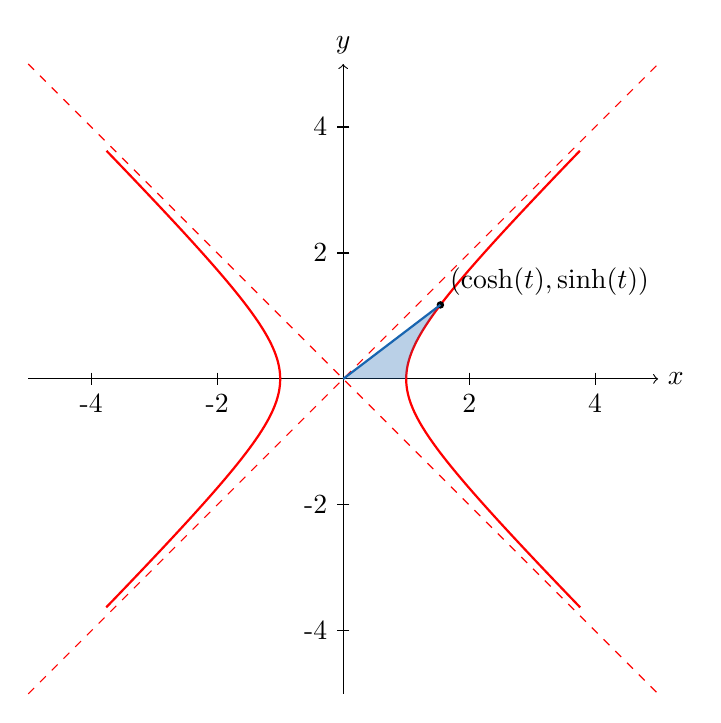
\begin{tikzpicture}[scale=0.8]
            % Draw the axes
            \draw[->] (-5, 0) -- (5, 0) node[right] {$x$};
            \draw[->] (0, -5) -- (0, 5) node[above] {$y$};
        
            % Draw ticks on the axes
            \foreach \x in {-4, -2, 2, 4}
                \draw (\x, 0.1) -- (\x, -0.1) node[below] {\x};
            \foreach \y in {-4, -2, 2, 4}
                \draw (0.1, \y) -- (-0.1, \y) node[left] {\y};
        
            % Draw the hyperbola branches
            \draw[thick, red, domain=-2:2, samples=100] plot ({cosh(\x)}, {sinh(\x)});
            \draw[thick, red, domain=-2:2, samples=100] plot ({-cosh(\x)}, {sinh(\x)});
        
            % Draw the asymptotes
            \draw[red, dashed] (-5, -5) -- (5, 5);
            \draw[red, dashed] (-5, 5) -- (5, -5);
        
            % Add a point on the hyperbola
            \coordinate (P) at ({cosh(1)}, {sinh(1)});
            \draw[fill] (P) circle (0.05) node[above right] {$(\cosh(t), \sinh(t))$};
        
            % Connect the labeled point to the origin
            \draw[thick, blue] (0, 0) -- (P);
        
            % Fill the sector area between hyperbola, line, and x-axis
            \fill[blue, opacity=0.3, domain=0:1, variable=\t]
                (0, 0) -- plot ({cosh(\t)}, {sinh(\t)}) -- cycle;
        \end{tikzpicture}
    \end{center}
    \caption{Sector of the hyperbola}
    \centering
\end{figure}
\paragraph{Catenary} The hyperbolic cosine function describes the shape of a hanging chain or cable. The catenary is the curve formed by a chain hanging from two points. It is given by the equation:
\begin{equation}
    a \cosh\left(\frac{x}{a}\right),
\end{equation}
\begin{definition}[Hyperbolic Tangent]
    The hyperbolic tangent function is defined as:
    \begin{equation}
        \tanh(x) = \frac{\sinh(x)}{\cosh(x)} = \frac{e^x - e^{-x}}{e^x + e^{-x}}. 
    \end{equation}
\end{definition}
\paragraph{Derivative} The derivative of the hyperbolic tangent function resembles the derivative of the regular tangent function:
\begin{equation} \frac{d}{dx} \tanh(x) = \text{sech}^2(x). \end{equation}
\paragraph{Identities} The hyperbolic tangent function satisfies the following identities:
\begin{align}
    \tanh(x) &= \frac{\sinh(x)}{\cosh(x)}, \\
    \text{sech}^2(x) &= 1 - \tanh^2(x).
\end{align}
\paragraph{Secant, Cosecant, Cotangent} The hyperbolic secant, cosecant, and cotangent functions are defined similarly to the regular secant, cosecant, and cotangent functions. They are the \textbf{reciprocal} of the hyperbolic cosine, sine, and tangent functions, respectively.
\paragraph{Inverse Hyperbolic Functions} The inverse hyperbolic functions are defined as the inverse of the hyperbolic functions. They are denoted by $\sinh^{-1}(x)$, $\cosh^{-1}(x)$, $\tanh^{-1}(x)$, etc.
\begin{align}
    \text{arsinh } x &= \ln\left(x + \sqrt{x^2 + 1}\right) \\[10pt]
    \text{arcosh } x &= \ln\left(x + \sqrt{x^2 - 1}\right) \\[10pt]
    \text{artanh } x &= \frac{1}{2} \ln\left(\frac{1 + x}{1 - x}\right) \\[10pt]
    \text{arcsch } x &= \ln\left(\frac{1}{x} + \sqrt{\frac{1}{x^2} + 1}\right) \\[10pt]
    \text{arsech } x &= \ln\left(\frac{1}{x} + \sqrt{\frac{1}{x^2} - 1}\right) \\[10pt]
    \text{arcoth } x &= \frac{1}{2} \ln\left(\frac{x + 1}{x - 1}\right)
\end{align}
\section{Further Applications of Integrals}
\subsection{Arc Length}
\paragraph{Arc Length}
    Given the curve $C: y = f(x)$, the arc length of the curve between two points $a$ and $b$, where $y'(x)$ is continuous, we would like the compute the arc length of the curve:
    $$ L = \int_C ds$$
\paragraph{Formula} We can derive the formula for the arc length of a curve $y = f(x)$ between two points $a$ and $b$ as:
\begin{align}
    \intertext{At $x_i$ and $x_{i+1}$, the length of the segment is:}
    \Delta s &\approx \sqrt{(x_{i+1} - x_i)^2 + (y_{i+1} - y_i)^2} \nonumber \\
            &= \sqrt{\Delta_i x^2 + \Delta_i y^2} \nonumber \\
    \intertext{We also have, by MVT:}
    \frac{\Delta y}{\Delta x} &= y'(c) \nonumber \\
    \Delta y &= y'(c) \Delta x \nonumber \\
    \Delta s &\approx \sqrt{\Delta x^2 + (y'(c) \Delta x)^2} \nonumber \\
            &= \sqrt{1 + y'(c)^2} \Delta x \nonumber \\
    \intertext{Taking a Riemann sum:}
    L &= \lim_{n \to \infty} \sum_{i=1}^n \sqrt{1 + y'(c_i)^2} \Delta x \nonumber \\
    &= \int_a^b \sqrt{1 + y'(x)^2} \, dx 
\end{align}
\begin{example}
    Given $f(x) = x^\frac{3}{2}$ between $x = 0$ and $x = 44$, we would like to compute the arc length of the curve:
    \begin{align*}
        L &= \int_0^{44} \sqrt{1 + \left(\frac{3}{2}x^{\frac{1}{2}}\right)^2} \, dx \\
        &= \int_0^{44} \sqrt{1 + \frac{9}{4}x} \, dx \\
        &= \frac{8}{27} \left(1 + \frac{9}{4}x\right)^{\frac{3}{2}} \Big|_0^{44} = 296
    \end{align*}
\end{example}
\paragraph{Inverse} Also, we can take $x = f^{-1}(y)$ to compute the arc length of a curve.
\begin{equation}
    L = \int_{f(a)}^{f(b)} \sqrt{1 + ((f{^{-1}})'(y))^2} \, dy
\end{equation}
\subsection{Surface Area of Revolution}
\paragraph{Surface Area of Revolution} Given the curve $C: y = f(x)$, we would like to compute the surface area of the curve between two points $a$ and $b$ when rotated about the $x$-axis:
    $$ A_x = \int_C 2\pi y \, ds$$
\paragraph{Formula} Deriving the formula for the surface area of a curve $y = f(x)$ between two points $a$ and $b$ rotated about the $x$-axis as follows:
\begin{align}
    \intertext{At $x_i$ and $x_{i+1}$, the length of the segment is:}
    \Delta s &\approx \sqrt{\Delta_i x^2 + \Delta_i y^2} \nonumber \\
    \intertext{The surface area of the segment is, by continuity:}
    A_i &= \pi (y_i + y_{i+1}) \Delta s = 2\pi y^\star \Delta s \quad 
    \intertext{As the difference between $y^\star$ and $y_i$ diminishes as $\Delta x \rightarrow 0$, taking a Riemann sum:}
    A_x &= \lim_{n \to \infty} \sum_{i=1}^n 2\pi y_i \sqrt{\Delta_i x^2 + \Delta_i y^2} \nonumber \\
    &= \int_a^b 2\pi y \sqrt{1 + y'(x)^2} \, dx
    \intertext{The surface area of a curve $y = f(x)$ (i.e. $x = f^{-1}$)between two points $f(a)$ and $f(b)$ rotated about the $y$-axis is:}
    A_y &= \int_{f(a)}^{f(b)} 2\pi x \sqrt{1 + x'(y)^2} \, dy
\end{align}
\begin{example}
    Given $y = \sqrt{x}$ between $x = 0$ and $x = 1$, we would like to compute the surface area of the curve:
    \begin{align*}
        A_x &= \int_0^1 2\pi \sqrt{x} \sqrt{1 + \frac{1}{4x}} \, dx \\
        &= \pi \int^1_0 \sqrt{4x + 1} \, dx \\
        \intertext{Let $u = 4x + 1$, then $du = 4dx$:}
        &= \frac{\pi}{4} \int^5_1 \sqrt{u} \, du \\
        &= \frac{\pi}{6}\left(5^\frac{3}{2} -1\right)
    \end{align*}
\end{example}
\subsection{Applications to Physics and Engineering}
\subsubsection{Hydrostatic Pressure and Force}
\paragraph{Hydrostatic Pressure} The hydrostatic pressure and Force is given by the Archimedes' principle:
\begin{subequations}
    \begin{align}
        P &= \rho g \cdot d, \\
        F &= \rho g \cdot d \cdot A
    \end{align}
\end{subequations}
\paragraph{Riemann Sum} Given a tank rectangular with width defined by $w = f(x)$, we can take a horizontal slice, $x^\star$, of the tank to compute the force exerted on the tank by the water:
\begin{equation}
    F =\sum_{i=1}^n \rho g x_i f(x_i) \Delta x
\end{equation}
\paragraph{Formula} Given a tank rectangular with width defined by $w = f(x)$, where $x$ is depth, we would like to compute the force exerted on the tank by the water:
\begin{equation}
    F = \int_0^b \rho g x f(x) \cdot dx
\end{equation}
, which is derived by considering $dx$ as the depth a horizontal slice of the tank.
\subsubsection{Center of Mass and Moments of Inertia}
\paragraph{Properties of the Center of Mass} The center of mass of a region $R$ has the following properties:
\begin{enumerate}
    \item \textbf{Symetry}: For all axis of symmetry, the center of mass lies on the axis.
    \item \textbf{Additivity}: The center of mass of a region is the weighted average of the centers of mass of its parts. The weights are the areas of the parts.
    \begin{equation}
        \bar{x} = \sum_i \frac{A_i\bar{x_i}}{A}
    \end{equation}
\end{enumerate}
\paragraph{Formula} The centroid of a uniformly-dense region $R$ bounded by $y=f(x),\,x\in[a,b],\,y\in[f(a),f(b)]$ is derived as follows:
\begin{align}
    \intertext{We first have $x_i^\star$ and $A_i$ as follows:}
    x_i^\star = \frac{1}{2}(x_i + x_{i+1}) &\quad A_i = f(x_i) \Delta x \nonumber \\
    \intertext{For $\bar{x}$, we have:}
    A\bar{x} &\approx \sum_i x_i^\star A_i \nonumber \\
    \intertext{Taking a Riemann sum:}
    A\bar{x} &= \lim_{n \to \infty} \sum_i x_i^\star A_i  \nonumber \\
    \bar{x} &= \frac{1}{A}\int_a^b x f(x) \, dx
    \intertext{Similarly, for $\bar{y}$:}
    A\bar{y} &= \lim_{n \to \infty} \sum_i f(x_i^\star) A_i \nonumber \\
    \bar{y} &= \frac{1}{A}\int_a^b \frac{1}{2}(f(x))^2 \, dx
\end{align}
\begin{theorem}[Pappus's Theorem]
    The volume of a solid of revolution is given by the product of the area of the region and the distance, $R$, traveled by the centroid of the region from the axis of rotation.
    \begin{equation}
        V = 2\pi R A
    \end{equation}
\end{theorem}
\begin{example}[Eliptical Torus]
    Given an eliptical torus (tall donut) with major axis $a$ and minor axis $b$, we would like to compute the volume of the torus:
    \begin{align*}
        V &= 2\pi R A \\
        &= 2\pi R \cdot \pi ab = 2\pi^2 abR
    \end{align*}
    This could be, alternatively, shown via the washer method and the shell method.
\end{example}
\subsection{Applications to Economics and Biology}
``Biologists are so bad at math'' - Prof. Davis as he proceeds to erase the board and skip to the next section.
\section{Parametric Equations and Polar Coordinates}
\subsection{Curves Defined by Parametric Equations}
\paragraph{Parametric Equations} For $t \in \mathbb{R}$, we have:
\begin{equation}
    x = x(t), \quad y = y(t)
\end{equation}
\begin{example}[Newton's Laws of Motion]
    Given $\ddot{x} = 0$, $\ddot{y} = -g$, we have:
    \begin{align*}
        x(t) &= A_1 t + A_2, \\
        y(t) &= -\frac{1}{2}gt^2 + B_1 t + B_2
    \end{align*}
    At initial conditions $t = 0$, we have $x(0) = 0$, $y(0) = 0$, $\dot x(0) = v_0 \cos(\theta)$, $\dot y(0) = v_0 \sin(\theta) - \frac{1}{2}gt^2$.
\end{example}
\begin{example}[Ellipse]
    Given $x = a\cos(t)$, $y = b\sin(t)$, we have:
    \begin{align*}
        x^2 &= a^2\cos^2(t), \\
        y^2 &= b^2\sin^2(t)
    \end{align*}
    , which satisfies $x^2/a^2 + y^2/b^2 = 1$.
\end{example}
\paragraph{Intersections of Parametric Curves} Given two parametric curves $C_1,\,C_2$, defined by:
\begin{align*}
    C_1:\, x_1 &= x_1(t), \quad y_1 = y_1(t) \\
    C_2:\, x_2 &= x_2(t), \quad y_2 = y_2(t)
\end{align*}
, we can find the intersection points by solving the system of equations:
\begin{align*}
    x_1(t) &= x_2(t) \\
    y_1(t) &= y_2(t)
\end{align*}
\begin{example}
    Given $x_1 = 2t+t$, $y_1 = 5-4t$, $x_2 = 3 - 5\cos(\pi t)$, $y_2 = 1 + 5\sin(\pi t)$, we have:
    \begin{align*}
        2t + 1 &= 3 - 5\cos(\pi t) \\
        5 - 4t &= 1 + 5\sin(\pi t)
    \end{align*}
\end{example}
\subsection{Calculus with Parametric Curves}
\paragraph{Tangents} The tangent to a parametric curve $C$ at a point $t$ is given by:
\begin{equation}
    \frac{dy}{dx} = \frac{dy/dt}{dx/dt} = \frac{y'(t)}{x'(t)}
\end{equation}
\paragraph{Equation of the Tangent} The equation of the tangent to a parametric curve $C$ at a point $t_0$ is given by:
\begin{equation}
    y'(t_0) (x-x(t_0)) - x'(t_0) (y-y(t_0)) = 0
\end{equation}
Hence, if $x'(t_0) = 0$, we have a vertical tangent; if $y'(t_0) = 0$, we have a horizontal tangent. However, if $x'(t_0) = 0$ and $y'(t_0) = 0$, we have no information.
\begin{example}
    Let $x = \sin 2t$, $y = \sin t$, we have:
    \begin{align*}
        x'(t) &= 2\cos 2t, \\
        y'(t) &= \cos t
    \end{align*}
    \textbf{Vertical Tangent}: $2\cos 2t = 0 \Rightarrow t = \frac{\pi}{4} + \frac{n\pi}{2}$.
    \textbf{Horizontal Tangent}: $\cos t = 0 \Rightarrow t = \frac{\pi}{2} + n\pi$.
    \textbf{At $t = 0$} we have $x' = y' = 0$. Thus, we have no information. On the graph, we see that the curve intersects itself at $t = 0$.
\end{example}
\paragraph{Area under Parametric Curve} The area under a parametric curve $C$ between $t_1$ and $t_2$ is given by:
\begin{equation}
    A = \int^{x(t_2)}_{x(t_1)} y(x) \, dx = \int_{t_1}^{t_2} y(t) x'(t) \, dt 
\end{equation}
\begin{definition}[Orientation]
    The orientation of a parametric curve $C$ is given by the direction of the curve as $t$ increases. If the enclosed area is to the left of the trace of $t$ (counter-clockwise) the orientation is positive; otherwise, it is negative.
\end{definition}
\paragraph{} The sign of the area of a parametric curve $C$ is given by the orientation of the curve.
\paragraph{Area of Closed Curves} The area of a closed parametric curve $C$ is given by:
\begin{equation}
    A = \oint_C dA = \int_{t_1}^{t_2} y(t) x'(t) \, dt = \int_{t_1}^{t_2} x(t) y'(t) \, dt
\end{equation}
, where
\begin{equation*}
    x(t_1) = x(t_2), \quad y(t_1) = y(t_2) \quad \text{and} \quad \text{$t_2$ is the smallest $t>t_1$ to satisfy the condition}.
\end{equation*}
\paragraph{Arc Length} The arc length of a parametric curve $C$ is given by:
\begin{equation}
    L = \int_a^b \sqrt{\left(\frac{dx}{dt}\right)^2 + \left(\frac{dy}{dt}\right)^2} \, dt
\end{equation}
\begin{example}
    Given $x = t\cos t$, $y = t\sin t$, we have:
    \begin{align*}
        \frac{dx}{dt} &= \cos t - t\sin t, \\
        \frac{dy}{dt} &= \sin t + t\cos t
    \end{align*}
    Thus, the arc length is given by:
    \begin{align*}
        L &= \int_0^{2\pi} \sqrt{(\cos t - t\sin t)^2 + (\sin t + t\cos t)^2} \, dt \\
        &= \int_0^{2\pi} \sqrt{1 + t^2} \, dt
        \intertext{Using the substitution $t = \tan \theta$, we have:}
        &= \pi \sqrt{1 + 4\pi^2} + \frac{1}{2}\ln(2\pi + \sqrt{1 + 4\pi^2})
    \end{align*}
\end{example}
\paragraph{Surface Area of Revolution} The surface area of a parametric curve $C$ rotated about the $x$-axis is given by:
\begin{align}
    A &= \int_a^b 2\pi y(t) ds \nonumber \\
    \intertext{From the arc length formula, we have $ds = \sqrt{(\frac{dx}{dt})^2 + (\frac{dy}{dt})^2} \, dt$, thus:}
    &= \int_a^b 2\pi y(t) \sqrt{\left(\frac{dx}{dt}\right)^2 + \left(\frac{dy}{dt}\right)^2} \, dt
\end{align}
Similarly, the surface area of a parametric curve $C$ rotated about the $y$-axis is given by:
\begin{equation}
    A = \int_a^b 2\pi x(t) \sqrt{\left(\frac{dx}{dt}\right)^2 + \left(\frac{dy}{dt}\right)^2} \, dt
\end{equation}
\begin{example}[Surface Area of of a Ellipse]
    Given $x = a\sin t$, $y = b\cos t$, we have:
    \begin{align*}
        \frac{dx}{dt} &= a\cos t, \\
        \frac{dy}{dt} &= -b\sin t
    \end{align*}
    Thus, the surface area of the ellipse is given by:
    \begin{align*}
        A &= \int_0^{2\pi} 2\pi b\cos t \sqrt{a^2\cos^2 t + b^2\sin^2 t} \, dt \\
        &= 2\pi b \int_0^{2\pi} \sqrt{a^2 (1 - \sin^2 t) + b^2 \sin^2 t} \, dt \\
        &= 2\pi b \int_0^{2\pi} \sqrt{a^2 + b^2 - (a^2 - b^2)\sin^2 t} \, dt
    \end{align*}
    This has no analytical solution, but can be solved numerically. Typically, we take $\epsilon = \sqrt{\frac{a^2-b^2}{a^2}}$.
\end{example}
\section{Polar Coordinates}
\paragraph{Polar Coordinates} Given a point $P$ in the plane, we can define the polar coordinates of $P$ as $(r, \theta)$, where $r$ is the distance from the origin to $P$ and $\theta$ is the angle between the positive $x$-axis and the line segment from the origin to $P$.
\paragraph{Transformation} We can convert between polar and Cartesian coordinates as follows:
\begin{equation}
    x = r\cos \theta, \quad y = r\sin \theta
\end{equation}
\paragraph{Reverse Transformation} We can convert between Cartesian and polar coordinates as follows:
\begin{equation}
    r = \sqrt{x^2 + y^2}, \quad \theta = \arctan\left(\frac{y}{x}\right)
\end{equation}
\paragraph{Note} The angle $\theta$ is not unique, as $\theta + 2\pi n$ for $n \in \mathbb{Z}$ represents the same point, beware of this when converting between polar and Cartesian coordinates.
\begin{example}[Lines]
    \begin{align*}
        y = mx + b &\implies \theta = \alpha = \arctan m \\
        x = a &\implies r = a\sec \theta \\
        y = a &\implies r = a\csc \theta
    \end{align*}
\end{example}
\begin{example}[Cirlces]
    \begin{align*}
        x^2 + y^2 = a^2 &\implies r = a \\
    \end{align*}
    Let $r = 6\sin \theta$, we have:
    \begin{align*}
        r^2 &= 6r\sin \theta \\
        x^2 + y^2 &= 6y \\
        x^2 + (y-3)^2 &= 9
    \end{align*}
    We deduce that the curve is a circle with radius $3$ and center $(0,3)$.
\end{example}
\paragraph{Cylinrical Coordinates} Given a point $P$ in space, we can define the cylindrical coordinates of $P$ as $(r, \theta, z)$, where $r$ is the distance from the $z$-axis to $P$, $\theta$ is the angle between the positive $x$-axis and the projection of the line segment from the origin to $P$ onto the $xy$-plane, and $z$ is the distance from the $xy$-plane to $P$.
\paragraph{Spherical Coordinates} Given a point $P$ in space, we can define the spherical coordinates of $P$ as $(\rho, \theta, \phi)$, where $\rho$ is the distance from the origin to $P$, $\theta$ is the angle between the positive $x$-axis and the projection of the line segment from the origin to $P$ onto the $xy$-plane, and $\phi$ is the angle between the positive $z$-axis and the line segment from the origin to $P$.
\subsection{Graphing in Polar Coordinates}
\begin{example}
    Let $r = \frac{1}{2} + \cos \theta$, we first figure out the origin of the curve by setting $r = 0$:
    \begin{align*}
        0 &= \frac{1}{2} + \cos \theta \\
        \theta &= \frac{2\pi}{3},\, \frac{4\pi}{3}
    \end{align*}
    We then deduce the maximum and minimum of the curve to the origin by setting $\frac{dr}{d\theta} = 0$:
    \begin{align*}
        \frac{dr}{d\theta} &= -\sin \theta = 0 \\
        \theta &= 0,\, \pi,\, 2\pi
    \end{align*}
    We also look for symmetry in the curve by checking $r(\theta) = r(-\theta)$:
    \begin{align*}
        \frac{1}{2} + \cos \theta &= \frac{1}{2} + \cos(-\theta) \\
    \end{align*}
    Thus, the curve is symmetric about the $x$-axis. We also look for symmetry about the $y$-axis by checking $r(\theta) = r(\pi + \theta)$:
    \begin{align*}
        \frac{1}{2} + \cos \theta \neq \frac{1}{2} + \cos(\pi + \theta) \\
    \end{align*}
    Thus, the curve is not symmetric about the $y$-axis. We also look for intervals in which the curve is increasing or decreasing by checking $r'(\theta) > 0$ or $r'(\theta) < 0$.
\end{example}
\paragraph{Common Polar Curves} Some common polar curves are:
\begin{enumerate}
    \item \textbf{Cardioid}: $r = a(1 + \cos \theta)$ (heart-shaped)
    \item \textbf{Circle}: $r = a\cos \theta$ 
    \item \textbf{Limasçons}: $r = a + b\sin \theta$ (heart with a hole)
    \item \textbf{Lemniscate}: $r^2 = a^2\sin 2\theta$ (infinity symbol, diagonal) \vspace{1em} $\quad r^2 = a^2\cos 2\theta$ (infinity symbol, horizontal)
    \item \textbf{Petal Curves}: $r = a\cos n\theta$ ($mn$-petal flower) \vspace{1em} $\quad r = a\sin n\theta$ ($mn$-petal flower); $m=2$ if $n$ is even, $m=1$ if $n$ is odd.
\end{enumerate}
\paragraph{} Below are some examples of polar curves:
\begin{figure}[h!]
    \centering
    \begin{minipage}{0.48\textwidth}
        \centering
        \begin{tikzpicture}[scale=1.5]
            \draw[->] (-2.5,0) -- (2.5,0) node[right]{$x$};
            \draw[->] (0,-2.5) -- (0,2.5) node[above]{$y$};
            \draw[domain=0:360, smooth, samples=100, red] plot ({(1+cos(\x))*cos(\x)}, {(1+cos(\x))*sin(\x)});
            \node at (0,-3) {Cardioid: $r = 1 + \cos \theta$};
        \end{tikzpicture}
    \end{minipage}
    \hfill
    \begin{minipage}{0.48\textwidth}
        \centering
        \begin{tikzpicture}[scale=1.5]
            \draw[->] (-2.5,0) -- (2.5,0) node[right]{$x$};
            \draw[->] (0,-2.5) -- (0,2.5) node[above]{$y$};
            \draw[domain=0:360, smooth, samples=100, blue] plot ({cos(\x)*cos(\x)}, {cos(\x)*sin(\x)});
            \node at (0,-3) {Circle: $r = \cos \theta$};
        \end{tikzpicture}
    \end{minipage}
\end{figure}

\begin{figure}[h!]
    \centering
    \begin{minipage}{0.48\textwidth}
        \centering
        \begin{tikzpicture}[scale=1.5]
            \draw[->] (-2.5,0) -- (2.5,0) node[right]{$x$};
            \draw[->] (0,-2.5) -- (0,2.5) node[above]{$y$};
            \draw[domain=0:360, smooth, samples=100, green] plot ({(1+0.5*sin(\x))*cos(\x)}, {(1+0.5*sin(\x))*sin(\x)});
            \node at (0,-3) {Limaçon: $r = 1 + 0.5\sin \theta$};
        \end{tikzpicture}
    \end{minipage}
    \hfill
    \begin{minipage}{0.48\textwidth}
        \centering
        \begin{tikzpicture}[scale=1.5]
            \draw[->] (-2.5,0) -- (2.5,0) node[right]{$x$};
            \draw[->] (0,-2.5) -- (0,2.5) node[above]{$y$};
            \draw[domain=0:360, smooth, samples=100, orange] plot ({sqrt(abs(sin(2*\x)))*cos(\x)}, {sqrt(abs(sin(2*\x)))*sin(\x)});
            \node at (0,-3) {Lemniscate: $r^2 = \sin 2\theta$};
        \end{tikzpicture}
    \end{minipage}
\end{figure}

\begin{figure}[h!]
    \centering
    \begin{minipage}{0.48\textwidth}
        \centering
        \begin{tikzpicture}[scale=1.5]
            \draw[->] (-2.5,0) -- (2.5,0) node[right]{$x$};
            \draw[->] (0,-2.5) -- (0,2.5) node[above]{$y$};
            \draw[domain=0:360, smooth, samples=100, purple] plot ({cos(3*\x)*cos(\x)}, {cos(3*\x)*sin(\x)});
            \node at (0,-3) {Petal Curve: $r = \cos 3\theta$};
        \end{tikzpicture}
    \end{minipage}
    \hfill
    \begin{minipage}{0.48\textwidth}
        \centering
        \begin{tikzpicture}[scale=1.5]
            \draw[->] (-2.5,0) -- (2.5,0) node[right]{$x$};
            \draw[->] (0,-2.5) -- (0,2.5) node[above]{$y$};
            \draw[domain=0:360, smooth, samples=100, brown] plot ({sin(2*\x)*cos(\x)}, {sin(2*\x)*sin(\x)});
            \node at (0,-3) {Petal Curve: $r = \sin 2\theta$};
        \end{tikzpicture}
    \end{minipage}
\end{figure}
\newpage
\paragraph{} \label{sec:polar} A detailed list of polar curves and their properties could be found in Appendix \ref{app:polarCurves}. 
\subsection{The intersection of Polar Curves}
\begin{example}
    Let $r_1 = \sin \theta$, $r_2 = -\cos \theta$, we have:
    \begin{align*}
        \sin \theta &= -\cos \theta \\
        \tan \theta &= -1 \\
        \theta &= \frac{3\pi}{4},\, \frac{7\pi}{4}
    \end{align*}
    At these points, we can find the $x$ and $y$ coordinates of the intersection points. But also, we must check for the origin point $(x,y) = (0,0)$. Also $r_1 = r_2$ is not always reliable so we have to check it intuitively.
\end{example}
\subsection{Area and Length in Polar Coordinates}
\paragraph{Area in Polar Coordinates} The area of a region $R: r = g(\theta)$ in polar coordinates is given by:
\begin{align}
    A &\approx \sum_{i} \frac{1}{2} [g(\theta_i)]^2 \Delta \theta_i \nonumber \\
    \intertext{Taking a Riemann sum:}
    &= \int_{\alpha}^{\beta} \frac{1}{2} [g(\theta)]^2 \, d\theta
\end{align}
\begin{example}
    Given $r = 1 + \cos \theta$, we have:
    \begin{align*}
        A &= \int_0^{2\pi} \frac{1}{2} (1 + \cos \theta)^2 \, d\theta \\
        &= \int_0^{2\pi} \frac{1}{2} (1 + 2\cos \theta + \cos^2 \theta) \, d\theta \\
        &= \frac{1}{2}\int_0^{2\pi} 2 + 2\cos \theta + \frac{1 + \cos 2\theta}{2} \, d\theta \\
        &= \frac{1}{2}\left(2\pi + 2\sin \theta + \frac{\theta}{2} + \frac{\sin 2\theta}{4}\right) \Big|_0^{2\pi}= \frac{3\pi}{2}
    \end{align*}
\end{example}
\paragraph{Area between Two Polar Curves} The area between two polar curves $r^2 = f(\theta)$ and $r = g(\theta)$ is given by:
\begin{equation}
    A = \int_{\alpha}^{\beta} \frac{1}{2} [f(\theta)^2 - g(\theta)^2] \, d\theta
\end{equation}
\begin{example}
    Given lemniscate $r^2 = 4\cos 2\theta$, circle $r = 1$, to find the area between the two curves, outside the circle, and inside the lemniscate. We have:
    \begin{align*}
        \intertext{We first consider the intersection points}
        4\cos 2\theta &= 1 \\
        \cos 2\theta &= \frac{1}{4} \\
        \intertext{We have points at $\theta = \pm 0.659$. Also, since the lemniscate is symmetric about the $y$-axis, we have:}
        \frac{1}{2}A &= \int_{-0.659}^{0.659} 4\cos^2 2\theta - 1 \, d\theta \\
        A &= 2.554
    \end{align*}
\end{example}
\begin{example}
    Given $r = \sin \theta$, $r = \cos \theta$, we have:
    \begin{align*}
        \intertext{We first consider the intersection points}
        \sin \theta &= \cos \theta \\
        \tan \theta &= 1 \\
        \theta &= \frac{\pi}{4}
        \intertext{We then consider the area between the two curves, notice that (0, 0) is also an intersection point.}
        A &= \frac{1}{2}\int_0^{\frac{\pi}{4}}  (\sin \theta)^2 - (\cos \theta)^2 \, d\theta \\
        &= \frac{\pi - 2}{8}
    \end{align*}
\end{example}
\paragraph{Tangent Lines in Polar Coordinates} The tangent line to a polar curve $r = r(\theta)$ is derived as follows:
\begin{align}
    x(\theta) &= r(\theta)\cos \theta, \quad y(\theta) = r(\theta)\sin \theta \nonumber \\
    \intertext{By chain rule, we have and product rule, we have:}
    \frac{dy}{dx} &= \frac{r'(\theta)\sin \theta + r(\theta)\cos \theta}{r'(\theta)\cos \theta - r(\theta)\sin \theta} \\
\end{align}
\paragraph{Length of a Polar Curve} Derived from above, the length of a polar curve $r = r(\theta)$ between $\alpha$ and $\beta$ is given by:
\begin{equation}
    L = \int_{\alpha}^{\beta} \sqrt{[r(\theta)]^2 + [r'(\theta)]^2} \, d\theta
\end{equation}
\begin{example}
    Given $r = a - a\cos \theta$, we have:
    \begin{align*}
        r' &= a\sin \theta \\
        L &= \int_0^{2\pi} \sqrt{(a - a\cos \theta)^2 + a^2\sin^2 \theta} \, d\theta \\
        &= a\int_0^{2\pi} \sqrt{2 - 2\cos \theta} \, d\theta \\
        \intertext{We can use the double angle formula to simplify the integral, with $\cos 2\theta = 1 - 2\sin^2 \theta$:}
        &= 8a
    \end{align*}
\end{example}
\section{Infinite Sequences and Series}
\subsection{Sequences}
\paragraph{Sequences} A sequence is a list of numbers written in a specific order.
\begin{example}
    Let $f: A \to \mathbb{R}$ be a function, and $f(x) = \frac{1}{x}$. We can restrict the domain of $f$ to $A = \{1, 2, 3, \ldots\} = \mathbb{N}$, and we can define the sequence $a_n = f(n) = \frac{1}{n}$.
\end{example}
\paragraph{Notation} Typcially, we denote a sequence as $\{a_n\}$, where $a_n$ is the $n$th term of the sequence. We can also denote with curly bracket as $\{a_n\} = \{a_1, a_2, a_3, \ldots\} = \{f(n)\}$.
\paragraph{Ratio} The ratio of two sequences $\{a_n\}$ and $\{b_n\}$ for some $n \le N$ is a sequence $\{c_n\}$ such that $c_n = \frac{a_n}{b_n}$.
\begin{example}
    Let $a_n = n^2$, $b_n = e^n$, we have:
    $$\frac{a_n}{b_n} = \{\frac{1}{e}, \frac{4}{e^2}, \frac{9}{e^3}, \ldots\}$$
\end{example}
\paragraph{Bounded Above} A sequence $\{a_n\}$ is said to be bounded above if there exists a number $M$ such that $|a_n| \le M$ for all $n$. (Similarly for bounded below).
\begin{definition}[Monotonic Sequences]
    A sequence $\{a_n\}$ is said to be non decreasing if $a_{n+1} \ge a_n$ for all $n$. Similarly, a sequence is said to be non increasing if $a_{n+1} \le a_n$ for all $n$. A sequence is said to be increasing if $a_{n+1} > a_n$ for all $n$. Similarly, a sequence is said to be decreasing if $a_{n+1} < a_n$ for all $n$.
\\ A sequence $\{a_n\}$ is said to be monotonic if it is either increasing, decreasing, non increasing, or non decreasing.
\end{definition}
\paragraph{Convergent Sequences} A sequence $\{a_n\}$ is said to be convergent if there exists a number $L$ such that for all $\epsilon > 0$, there exists an $N$ such that $|a_n - L| < \epsilon$ for all $n \ge N$.
\appendix
\newpage
\rhead{Calc II Appendix}
\lhead{\leftmark}
\pagenumbering{alph}
\section{Trigonometric Derivatives}
$$
\setlength{\tabcolsep}{8pt} % Adjust column spacing
\renewcommand{\arraystretch}{1.5} % Adjust row spacing
\begin{array}{|l|l|}
\hline
\textbf{Trigonometric Function} & \textbf{Inverse Trigonometric Function} \\ \hline
\dfrac{d}{dx} \text{sin}(x) = \text{cos}(x) & \dfrac{d}{dx} \text{arcsin}(x) = \dfrac{1}{\sqrt{1 - x^2}} \\ \hline
\dfrac{d}{dx} \text{cos}(x) = -\text{sin}(x) & \dfrac{d}{dx} \text{arccos}(x) = \dfrac{-1}{\sqrt{1 - x^2}} \\ \hline
\dfrac{d}{dx} \text{tan}(x) = \text{sec}^2(x) & \dfrac{d}{dx} \text{arctan}(x) = \dfrac{1}{1 + x^2} \\ \hline
\dfrac{d}{dx} \text{cot}(x) = -\text{csc}^2(x) & \dfrac{d}{dx} \text{arccot}(x) = \dfrac{-1}{1 + x^2} \\ \hline
\dfrac{d}{dx} \text{sec}(x) = \text{sec}(x)\text{tan}(x) & \dfrac{d}{dx} \text{arcsec}(x) = \dfrac{1}{|x|\sqrt{x^2 - 1}} \\ \hline
\dfrac{d}{dx} \text{csc}(x) = -\text{csc}(x)\text{cot}(x) & \dfrac{d}{dx} \text{arccsc}(x) = \dfrac{-1}{|x|\sqrt{x^2 - 1}} \\ \hline
\hline
\textbf{Hyperbolic Function} & \textbf{Inverse Hyperbolic Function} \\ \hline
\dfrac{d}{dx} \text{sinh}(x) = \text{cosh}(x) & \dfrac{d}{dx} \text{arsinh}(x) = \dfrac{1}{\sqrt{x^2 + 1}} \\ \hline
\dfrac{d}{dx} \text{cosh}(x) = \text{sinh}(x) & \dfrac{d}{dx} \text{arcosh}(x) = \dfrac{1}{\sqrt{x^2 - 1}} \quad (x > 1) \\ \hline
\dfrac{d}{dx} \text{tanh}(x) = \text{sech}^2(x) & \dfrac{d}{dx} \text{artanh}(x) = \dfrac{1}{1 - x^2} \quad (|x| < 1) \\ \hline
\dfrac{d}{dx} \text{coth}(x) = -\text{csch}^2(x) & \dfrac{d}{dx} \text{arcoth}(x) = \dfrac{1}{1 - x^2} \quad (|x| > 1) \\ \hline
\dfrac{d}{dx} \text{sech}(x) = -\text{sech}(x)\text{tanh}(x) & \dfrac{d}{dx} \text{arsech}(x) = \dfrac{-1}{x\sqrt{1 - x^2}} \quad (0 < x \leq 1) \\ \hline
\dfrac{d}{dx} \text{csch}(x) = -\text{csch}(x)\text{coth}(x) & \dfrac{d}{dx} \text{arcsch}(x) = \dfrac{-1}{|x|\sqrt{x^2 + 1}} \\ \hline
\end{array}
$$
\newpage
\section{Polar Curves}\label{app:polarCurves}
\paragraph{} Below are some common polar curves:
\begin{figure}[h!]
    \centering
    \includegraphics[width=0.9\textwidth]{AppendixItems/polarCurves.png}
    \caption{Polar Curves}
    \label{fig:polarCurves}
\end{figure}
Click: \ref{sec:polar} to go back to the section on polar coordinates.
\newpage
\section{Trigonometric Identities}\label{app:trigIdentities}
\begin{table}
    \centering
    \begin{tabular}{|c|c|}
        \hline
        \textbf{Identity} & \textbf{Value} \\
        \hline
        $\sin^2\theta + \cos^2\theta = 1$ & $1$ \\
        $\tan^2\theta = \sec^2\theta$ - 1 & $\sec^2\theta - 1$ \\
        $\tan\theta = \frac{\sin\theta}{\cos\theta}$ & $\frac{\sin\theta}{\cos\theta}$ \\
        $\cot\theta = \frac{\cos\theta}{\sin\theta}$ & $\frac{\cos\theta}{\sin\theta}$ \\
        $\sec\theta = \frac{1}{\cos\theta}$ & $\frac{1}{\cos\theta}$ \\
        $\csc\theta = \frac{1}{\sin\theta}$ & $\frac{1}{\sin\theta}$ \\
        $\sin(-\theta) = -\sin\theta$ & $-\sin\theta$ \\
        $\cos(-\theta) = \cos\theta$ & $\cos\theta$ \\
        $\tan(-\theta) = -\tan\theta$ & $-\tan\theta$ \\
        $\cot(-\theta) = -\cot\theta$ & $-\cot\theta$ \\
        $\sec(-\theta) = \sec\theta$ & $\sec\theta$ \\
        $\csc(-\theta) = -\csc\theta$ & $-\csc\theta$ \\
        $\sin(\theta \pm \phi) = \sin\theta\cos\phi \pm \cos\theta\sin\phi$ & $\sin\theta\cos\phi \pm \cos\theta\sin\phi$ \\
        $\cos(\theta \pm \phi) = \cos\theta\cos\phi \mp \sin\theta\sin\phi$ & $\cos\theta\cos\phi \mp \sin\theta\sin\phi$ \\
        $\tan(\theta \pm \phi) = \frac{\tan\theta \pm \tan\phi}{1 \mp \tan\theta\tan\phi}$ & $\frac{\tan\theta \pm \tan\phi}{1 \mp \tan\theta\tan\phi}$ \\
        $\sin(2\theta) = 2\sin\theta\cos\theta$ & $2\sin\theta\cos\theta$ \\
        $\cos(2\theta) = \cos^2\theta - \sin^2\theta$ & $\cos^2\theta - \sin^2\theta$ \\
        $2\cos(2\theta) = 2\cos^2\theta - 1 = 1 - 2\sin^2\theta$ & $2\cos^2\theta - 1 = 1 - 2\sin^2\theta$ \\
        $\tan(2\theta) = \frac{2\tan\theta}{1 - \tan^2\theta}$ & $\frac{2\tan\theta}{1 - \tan^2\theta}$ \\
        \hline
    \end{tabular}
    \caption{Trigonometric Identities}
    \label{tab:trigIdentities}
\end{table}
\end{document}
